\paragraph{\indent Актуальность темы.} Областью исследования работы является искусственный интеллект. Этот термин из года в год становится всё более популярным. На рисунке~\cref{fig:wordstat_dynamics} изображена динамика количества запросов <<искусственный интеллект>> в поисковой системе Яндекс в абсолютном и процентном отношении за последние шесть лет, а на рисунке~\cref{fig:google_trends_dynamics}~---~популярность темы <<Artificial intelligence (field of study)>> в сервисе Google Trends за последние два с половиной года, измеренная по внутренней технологии на основе количества поисковых запросов в поисковой системе Google и нормированная на пик популярности в выбранном промежутке времени.

\begin{figure}[b]
    \centerfloat{
        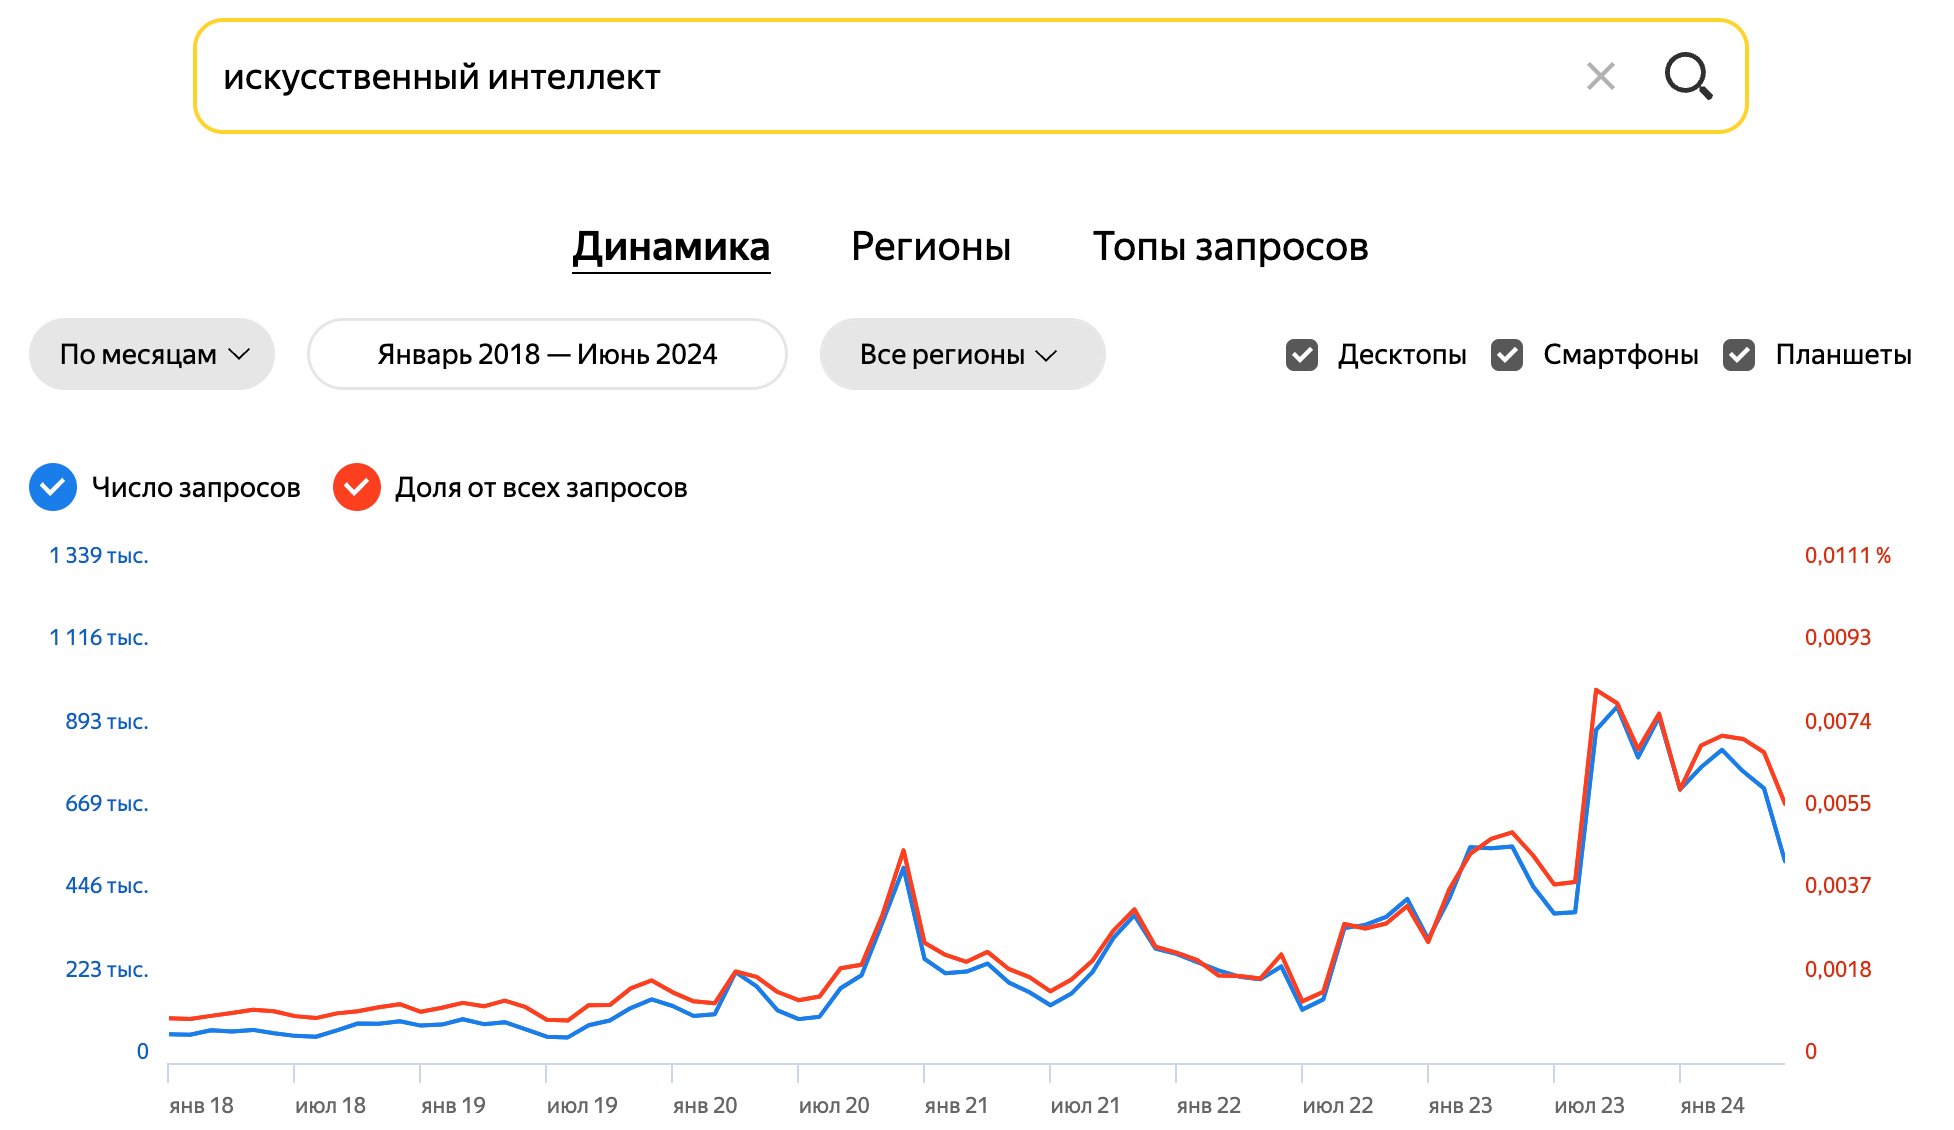
\includegraphics[width=\linewidth]{wordstat_dynamics}
    }
    \caption{Динамика общего количества запросов <<искусственный интеллект>> и их процентного отношения относительно всех запросов в поисковой системе Яндекс. График построен на основе значений из таблицы~\cref{tab:wordstat_dynamics} приложения~\cref{app:A1}}\label{fig:wordstat_dynamics}
\end{figure}

\begin{figure}[t]
    \centerfloat{
        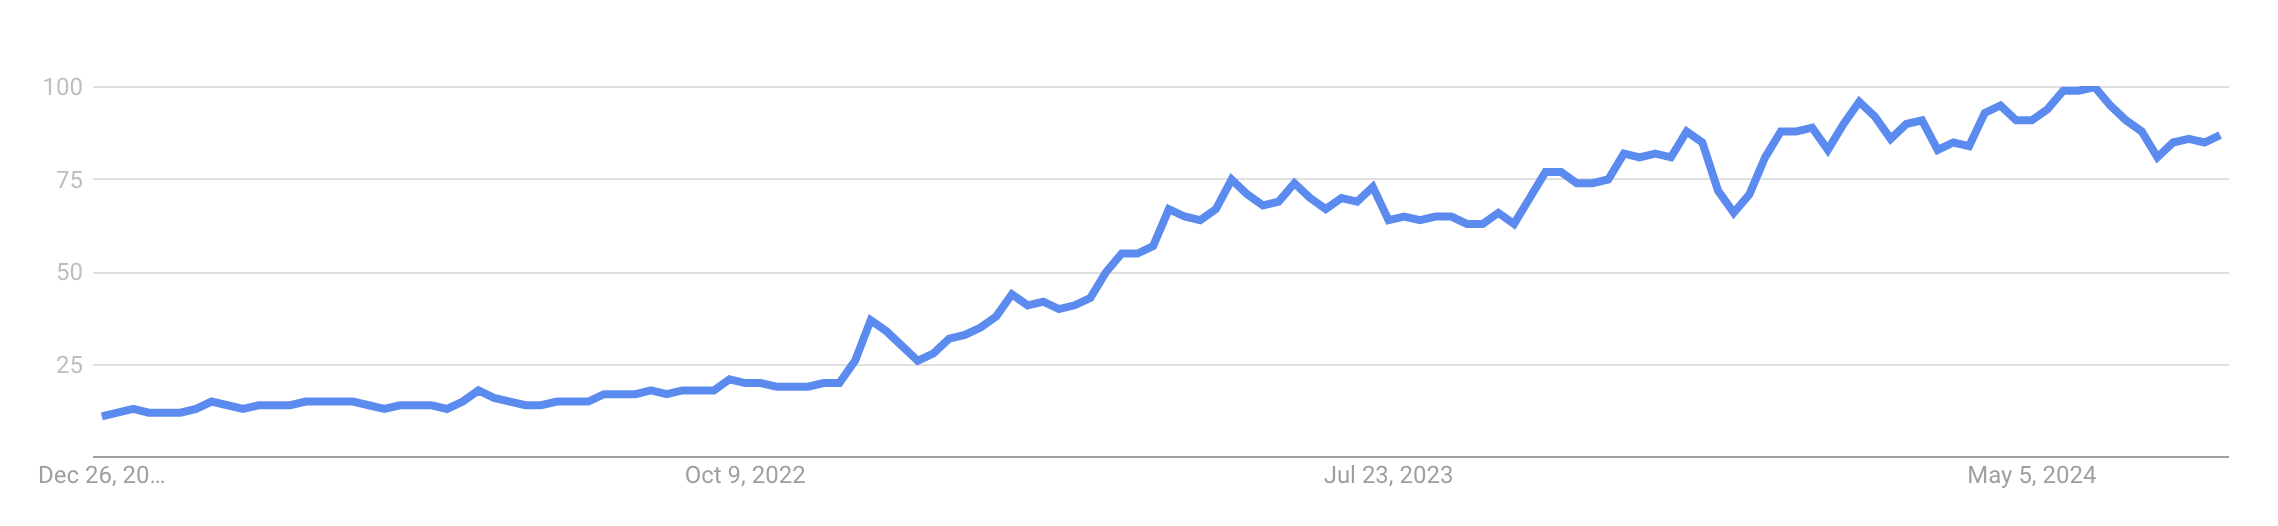
\includegraphics[width=\linewidth]{google_trends_dynamics}
    }
    \caption{Динамика популярности темы искусственного интеллекта в поисковой системе Google. График построен на основе значений из таблицы~\cref{tab:google_trends_dynamics} приложения~\cref{app:A2}}\label{fig:google_trends_dynamics}
\end{figure}

Однако, несмотря на растущую популярность этого явления, единого общепризнанного формального научного определения для него не сформулировано, хотя в литературе встречается множество его различных трактовок. Например, в словаре английского языка Collins English Dictionary, по версии которого аббревиатура AI (в переводе ИИ, искусственный интеллект) признана <<словом года>> по итогам 2023 г., даются следующие определения для этого термина (приведены на языке оригинала)~\cite{collins}:
\begin{enumerate}
    \item (Uncountable noun) artificial intelligence is a type of computer technology which is concerned with making machines work in an intelligent way, similar to the way that the human mind works. The abbreviation AI is also used.
    \item (Countable noun) an artificial intelligence is a computer system that has some of the same qualities as a human brain.
\end{enumerate}

Обращаясь к российским источникам, в Большой Российской энциклопедии встречается следующее определение~\cite{osipov}: искусственный интеллект (ИИ; англ. artificial intelligence, AI)~---~раздел информатики, в котором разрабатываются методы и средства компьютерного решения интеллектуальных задач, традиционно решаемых человеком. К прикладным направлениям ИИ относят создание технических устройств, способных к логическим выводам и рациональному поведению, к приобретению новых знаний и диалогу с человеком-пользователем. В теории ИИ используются математические методы, методы структурной лингвистики и когнитивной науки. 

В другом источнике можно встретить ещё несколько вариантов трактования определения ИИ~\cite[с.~247]{averkin}. Там же~\cite[с.~245]{averkin} подчёркивается неоднозначность терминологии в этой области, обусловленная высокими темпами её развития и индивидуальностью восприятия некоторых общеупотребимых терминов различными специалистами. Впервые термин был введён Джоном Маккарти в 1956 году на организованной им в Дартмутском колледже первой конференции (многодневном семинаре) по ИИ~\cite{osipov}. Годом позже Франком Розенблаттом была предложена математическая модель процесса восприятия~---~перцептрона~\cite{rosenblatt}, на основане которой впоследствии были разработаны нейронные сети, используемые для решения широкого спектра прикладных задач по сей день~\cite{skansi, nikolenko, trask, goodfellow, sharifani, sarkerdl, hoffer, zeiler}. 

По мере развития компьютерных технологий, прикладные интеллектуальные системы становились всё более комплексными и способными решать всё более сложные задачи. Сегодня искусственный интеллект используется в различных областях жизнедеятельности человека, в их числе: здравоохранение~\cite{glicksberg, awasthi, kitsios, elyan}, военная сфера~\cite{morgan, elmokadem}, сельское хозяйство~\cite{oliveira, bhagat, padhiary, wang}, финансовая сфера~\cite{bahoo, weber, shiyyab, shabsigh}, торговля и электронная коммерция~\cite{bawack, goti, ziakis}, транспортные потоки~\cite{sayed, jiang, mushtaq, loce}, умные города~\cite{wolniak, podda, zamponi, fekriershad}, кибербезопасность~\cite{malatji, ramanpreet, polito}, обработка естественного языка~\cite{zubiaga, khurana, alqahtani}, 3D-печать~\cite{kong, senthilnathan, petsiuk, paraskevoudis}, искусство~\cite{zhou, oksanen, watiktinnakorn} и другие. Помимо области применения, существуют и другие классификации ИИ~\cite{russell}.
\begin{itemize}[label=\textbullet]
    \item По уровню интеллекта. \begin{enumerate}
        \item Слабый ИИ: узкоспециализированный ИИ, который предназначен для выполнения одной конкретной задачи или набора задач. Примеры включают голосовых помощников~\cite{yang, huang, liu}, системы распознавания лиц~\cite{jha, ali, adjabi} и рекомендательные системы~\cite{azeroual, roy, zhang}.
        \item Сильный (общий) ИИ: ИИ, способный понимать, учиться и применять знания в различных областях, подобно человеческому интеллекту. На данный момент такой ИИ не существует и является целью долгосрочных исследований~\cite{buttazzo, butz, hoffmann}.
    \end{enumerate}
    \item По функциональным возможностям. \begin{enumerate}
        \item Реактивные машины: простейший вид ИИ, который реагирует на конкретные входные данные без сохранения опыта и памяти. Пример: Deep Blue, шахматный компьютер IBM~\cite{newborn}.
        \item Системы с ограниченной памятью: ИИ, который может использовать прошлый опыт для принятия решений, но не обладает долговременной памятью. Пример: автономные автомобили, которые используют прошлые данные для улучшения навигации и избегания препятствий~\cite{lai, padmaja, mahmoud, liy}.
        \item Теория разума: будущие системы ИИ, которые будут способны понимать и моделировать мысли, эмоции и социальные взаимодействия. Эти системы все еще находятся на стадии исследований и разработок~\cite{cuzzolin, williams}.
        \item Самосознание: самый продвинутый уровень ИИ, при котором система обладает самосознанием и осознанием своего существования. Это гипотетическая концепция, пока не реализованная на практике~\cite{chella, li, butlin}.
    \end{enumerate}
    \item По используемым подходам. \begin{enumerate}
        \item Символический (логический) ИИ: подход, основанный на использовании правил и логических операций для имитации человеческого мышления и принятия решений. Этот подход был доминирующим на ранних этапах развития ИИ и до сих пор находит применение в таких областях, как экспертные системы~\cite{calegari, belle, luo} и обработка естественного языка~\cite{hamilton, liuz, aithal}.
        \item Машинное обучение: подход, основанный на способности системы самостоятельно обучаться на основе данных, выявляя скрытые закономерности и зависимости~\cite{joshi, brink, vorontsov, wolf, muller, sarkerml}. Методы, основанные на машинном обучении применяются в широком спектре задач, от распознавания образов~\cite{bishop, singh, fieguth, braga-neto} до предсказательной аналитики~\cite{sghir, sharma, manasa, vjugin}.
        \item Эволюционные (генетические) алгоритмы: алгоритмы, основанные на процессе естественного отбора, использующие такие механизмы, как репродукция (воспроизводство), рекомбинация, мутация и отбор. Алгоритмы этой категории применяются в задачах оптимизации и поиска~\cite{alhijawi, katoch, khan, whitley, dejong, fraser1, fraser2, baricelli57, baricelli62}.
    \end{enumerate}
\end{itemize}
Принципы классификации систем ИИ в Российской Федерации определены в национальном стандарте ГОСТ Р 59277–2020~\cite{gost}.

Спектр областей применения ИИ разнообразен, однако в рамках данной работы будут рассмотрены только задачи из области машинного обучения, которые формально задаются следующим образом: пусть~$X$ и~$Y$~---~два алгебраических пространства и пусть существует некоторая неизвестная целевая зависимость между ними~$\hat{y} : X \to Y$; задачей является разработка отображения~$y : X \to Y$, которое наиболее точно приближало бы~$\hat{y}$ на всём множестве~$X$ по соответствующим значениям в пространстве~$Y$.

Пространство $X$ называют исходными данными. Данные представляют собой набор фактов, наблюдений, измерений или записей, которые можно анализировать для извлечения информации, получения знаний и принятия обоснованных решений. Данные могут быть собраны из различных источников, например, датчиков, баз данных, веб-сайтов, социальных сетей, электронных таблиц. Данные делятся на структурированные, полуструктурированные и неструктурированные. 
\begin{enumerate}
    \item Структурированные данные организованы в формате, который легко читать и анализировать с помощью компьютеров, как правило, в форме таблиц с чётко определенными столбцами и строками. Примеры: Таблицы в реляционных базах данных, CSV-файлы, электронные таблицы Excel.
    \item Полуструктурированные данные не соответствуют формальной структуре таблиц или баз данных, но всё же содержат организованную информацию с метками, которые облегчают анализ. Примеры: XML, JSON или YAML файлы.
    \item Неструктурированные данные не имеют определенной структуры и часто требуют значительной обработки для извлечения информации. Примеры: Тексты из социальных сетей, аудио и видеофайлы, изображения, записи разговоров.
\end{enumerate}

Область знаний, имеющая дело с данными, называется наукой о данных. Она объединяет в себе методы и подходы из теории вероятностей, математической статистики, машинного обучения и других областей~\cite{cao, holland}. Впервые этот термин был введён Петером Науром в книге «Краткий обзор компьютерных методов»~\cite{naur} в 1974 году. Единицей измерения информации, которую в данном контексте и называют данными, является бит. Этот термин впервые был упомянут в научной литературе в работе Клода Шеннона «Математическая теория связи»~\cite{shannon} в 1948 году, однако считается, что впервые был введён американским учёным-статистиком Джоном Тьюки годом ранее. В 1703 году в работе «Объяснение двоичной арифметики» (изданную в 1863 году~\cite{leibniz}) Лейбниц пишет, что двоичная система счисления была описана китайским императором и философом по имени Фу Си, который жил более чем за 4000 лет до Лейбница. Краткого современного названия китайский двоичный разряд (инь-янь, китайский бит) в то время пока ещё не имел. Китайский двубит (сы-сян), образующий четыре диграммы, и китайский трибит (ба-гуа), образующий восемь преднебесных и посленебесных триграмм, в современной международной терминологии собственных названий до сих пор не имеют. Один бит информации~---~это любой объект, который может принимать одно из двух возможных состояний. В Российской Федерации обозначения бита, а также правила его применения и написания установлены «Положением о единицах величин, допускаемых к применению в Российской Федерации»~\cite{law}. Для образования кратных единиц применяется с приставками СИ и с двоичными приставками. Появление бита позволило человеку моделировать информацию последовательностями нулей и единиц, работать с большими объёмами такой информации, анализировать их и делать на основе анализа выводы.

Пространство $Y$ называется целевым и представляет из себя множество ответов на задачу. Выбор вида пространств $X$ и $Y$ является необходимой частью постановки любой задачи машинного обучения. Для лучшего понимания рассмотрим несколько примеров типовых задач и для каждой из них высокоуровнево опишем вид этих пространств.
\begin{enumerate}
    \item Задача бинарной классификации (например, определение спама~\cite{hadi, adnan}).
    \begin{itemize}[label=\textbullet]
        \item Пространство $X$: Векторы признаков электронных писем, где каждый признак может быть числовым (например, количество слов) или категориальным (например, наличие определённых слов).
        \item Пространство $Y$: Множество $\left\{0, 1\right\}$, где 0 означает <<не спам>>, а 1 – <<спам>>.
    \end{itemize}
    
    \item Задача линейной регрессии (например, предсказание цены недвижимости~\cite{yazdani, sharmah, yadav}).
    \begin{itemize}[label=\textbullet]
        \item Пространство $X$: Векторы признаков недвижимости, включающие такие характеристики, как площадь, количество комнат, возраст дома и местоположение.
        \item Пространство $Y$: Непрерывное множество вещественных чисел $\mathbb{R}$, представляющее цену недвижимости.
    \end{itemize}
    
    \item Задача многоуровневой классификации (например, распознавание рукописных цифр~\cite{sultana, siddique, pashine}).
    \begin{itemize}[label=\textbullet]
        \item Пространство $X$: Векторы признаков изображений, представленных в виде пикселей. Например, для изображений размером $28 \times 28$ пикселей это будет вектор длиной 784.
        \item Пространство $Y$: Множество $\left\{0, 1, 2, 3, 4, 5, 6, 7, 8, 9\right\}$, где каждое значение соответствует определённой цифре.
    \end{itemize}
    
    \item Задача машинного перевода (например, перевод текста с английского на французский~\cite{zhangj, lyu}).
    \begin{itemize}[label=\textbullet]
        \item Пространство $X$: Последовательности слов в исходном языке (английский), представленные как последовательности векторов (векторов слов или эмбеддингов).
        \item Пространство $Y$: Последовательности слов в целевом языке (французский), также представленные как последовательности векторов.
    \end{itemize}
    
    \item Задача обучения с подкреплением (например, обучение робота передвижению~\cite{han, liz, zhangd, machado}).
    \begin{itemize}[label=\textbullet]
        \item Пространство $X$: Пространство состояний среды, в котором находится робот. Состояние может включать координаты робота, его скорость, ориентацию и другие параметры.
        \item Пространство $Y$: Пространство действий, которые может предпринимать робот, например, двигаться вперёд, поворачивать влево или вправо.
    \end{itemize}
\end{enumerate}

Зачастую исходное пространство данных является избыточным, из-за высокой мультикорреляции данных прогностическая модель $y$ оказывается неустойчивой. Для решения этой проблемы вводится абстрактное пространство $H$, называемое скрытым пространством, и рассматриваются методы снижения размерности исходных данных~\cite{isachenko} $f : X \to H, \: \dim H \ll \dim X$; после чего простая, устойчивая и точная модель $y$ строится уже на разреженном пространстве признаков: $y : H \to Y$. Подобласть науки о данных, изучающая процессы обнаружения скрытых, ранее неизвестных и потенциально полезных шаблонов и знаний в больших объемах данных, называется интеллектуальным анализом данных~\cite{fulkerson, franklin, barber, altun}.

В последние годы особый интерес для исследователей в области интеллектуального анализа данных и машинного обучения представляют фундаментальные (базовые) модели. Эти модели представляют собой, как правило, крупномасштабные нейронные сети, обученные на обширных наборах данных. Они используются для решения широкого спектра задач либо вообще без необходимости специализированного обучения под каждую, либо с минимальным дообучением под эти задачи, значительно менее вычислительно затратным, чем обучение самой базовой модели. Примерами в области обработки естественного языка являются GPT~\cite{brown, radford19, radford18}, разработанный OpenAI, и BERT~\cite{devlin}, созданный Google. Эти модели представляют из себя части нейронной сети, которая называется трансформером~\cite{vaswani}, обученные на большом количестве неразмеченных текстовых данных. Они продемонстрировали выдающиеся результаты в различных тестах и задачах, подтвердив потенциал фундаментальных моделей. Помимо обработки естественного языка такие модели используются и в других задачах~\cite{ren, miller, ma, moor}.

Направление интеллектуального анализа данных, имеющее дело с визуальными исходными данными, называется компьютерным зрением. В задачах компьютерного зрения элементы исходного пространства $X$ могут представлять из себя, например, изображения: цифровые фотографии, медицинские изображения, спутниковые и аэрофотоснимки; видео: кинематографические, телевизионные, спортивные трансляции, записи с камер видеонаблюдения; другие визуальные данные: трёхмерные облака точек, модели поверхностей, глубинные и инфракрасные изображения, текстурные карты. Компьютерное зрение решает широкий спектр задач, связанных с анализом и интерпретацией визуальной информации, среди них: обнаружение объектов на изображениях~\cite{chen, kaur, liul, xiao, lin, felzenszwalb, girshickr, girshick, rens, hek, liuw, redmon}, сегментация изображений~\cite{csurka, soylu, wangy, mittal, jiangb}, анализ сцены~\cite{wangx, valipoor, fan}, 3D-реконструкция~\cite{zhoul, samavati, hanxf, ham}, трекинг (отслеживание) объектов на видео~\cite{hassan, kadam, dong}, анализ движения~\cite{kaushik, hesse, colyer}, распознавание типов объектов~\cite{khalil, chatterjee, uijlings, vizilter, sebryakov}, распознавание текста~\cite{moudgil, ranjan, islam} и другие~\cite{davies, prince, szeliski, jain}. В задачах компьютерного зрения также используются фундаментальные модели~\cite{awais, wangw}. Одним из примеров фундаментальных моделей для компьютерного зрения является модель, обученная на ImageNet, крупномасштабном наборе данных, содержащем миллионы изображений, классифицированных по тысячам категорий~\cite{krizhevsky}. Модели, обученные на ImageNet, такие как ResNet~\cite{he, xie}, VGG~\cite{simonyan} и Inception~\cite{szegedy}, служат основой для разработки специализированных решений в области компьютерного зрения. Веса, полученные в процессе обучения на ImageNet, часто используются в качестве начальной точки для последующего дообучения на более специфичных наборах данных. Этот подход позволяет значительно сократить время и вычислительные ресурсы, необходимые для обучения моделей, а также улучшить их производительность на новых задачах, таких как детекция объектов, сегментация изображений, распознавание лиц и других.

Одной из сложных и интересных задач компьютерного зрения является мультикамерный трекинг, который включает в себя три взаимосвязанных компонента: детекцию объектов, трекинг и повторную идентификацию~\cite{zulfiqar, hu, hou, xu, ristani, narayan, wangxi, huangt, zajdel, gheissari, yi, liw, xuy, zheng, zhengl, sun, wangg, zhengm, wei, karanam, xiaot, zhenglia, mal, zhengs, kawanishi, figueira, layne, wangt, das, liwei2, liwei1, bialkowski, martinel, wangs, hirzer, baltieri, cheng, loy, zhengw, schwartz, gray, hermans, almazan, matsukawa, ristanie, zhengli}. Эта задача направлена на отслеживание движения объектов через несколько камер, что требует точного обнаружения объектов на каждом кадре, определения их траекторий и повторной идентификации объектов при переходе между камерами или при временной утрате видимости. Эта задача будет подробно рассмотрена в рамкой данной работы, в качестве объектов будут рассмотрены изображения людей в полный рост. Будет предложена адекватная комплексная мера оценки качества, а также предложено решение, основывающееся на фундаментальной человеко-центричной модели компьютерного зрения и демонстрирующее высокие точность и полноту распознавания при адекватной скорости работы в сравнении с другими методами решения этой задачи.



% {\actuality} Обзор, введение в тему, обозначение места данной работы в
% мировых исследованиях и~т.\:п., можно использовать ссылки на~другие
% работы~\autocite{Gosele1999161,Lermontov}
% (если их~нет, то~в~автореферате
% автоматически пропадёт раздел <<Список литературы>>). Внимание! Ссылки
% на~другие работы в~разделе общей характеристики работы можно
% использовать только при использовании \verb!biblatex! (из-за технических
% ограничений \verb!bibtex8!. Это связано с тем, что одна
% и~та~же~характеристика используются и~в~тексте диссертации, и в
% автореферате. В~последнем, согласно ГОСТ, должен присутствовать список
% работ автора по~теме диссертации, а~\verb!bibtex8! не~умеет выводить в~одном
% файле два списка литературы).
% При использовании \verb!biblatex! возможно использование исключительно
% в~автореферате подстрочных ссылок
% для других работ командой \verb!\autocite!, а~также цитирование
% собственных работ командой \verb!\cite!. Для этого в~файле
% \verb!common/setup.tex! необходимо присвоить положительное значение
% счётчику \verb!\setcounter{usefootcite}{1}!.

% Для генерации содержимого титульного листа автореферата, диссертации
% и~презентации используются данные из файла \verb!common/data.tex!. Если,
% например, вы меняете название диссертации, то оно автоматически
% появится в~итоговых файлах после очередного запуска \LaTeX. Согласно
% ГОСТ 7.0.11-2011 <<5.1.1 Титульный лист является первой страницей
% диссертации, служит источником информации, необходимой для обработки и
% поиска документа>>. Наличие логотипа организации на~титульном листе
% упрощает обработку и~поиск, для этого разметите логотип вашей
% организации в папке images в~формате PDF (лучше найти его в векторном
% варианте, чтобы он хорошо смотрелся при печати) под именем
% \verb!logo.pdf!. Настроить размер изображения с логотипом можно
% в~соответствующих местах файлов \verb!title.tex!  отдельно для
% диссертации и автореферата. Если вам логотип не~нужен, то просто
% удалите файл с~логотипом.

% \ifsynopsis
% Этот абзац появляется только в~автореферате.
% Для формирования блоков, которые будут обрабатываться только в~автореферате,
% заведена проверка условия \verb!\!\verb!ifsynopsis!.
% Значение условия задаётся в~основном файле документа (\verb!synopsis.tex! для
% автореферата).
% \else
% Этот абзац появляется только в~диссертации.
% Через проверку условия \verb!\!\verb!ifsynopsis!, задаваемого в~основном файле
% документа (\verb!dissertation.tex! для диссертации), можно сделать новую
% команду, обеспечивающую появление цитаты в~диссертации, но~не~в~автореферате.
% \fi

% % {\progress}
% % Этот раздел должен быть отдельным структурным элементом по
% % ГОСТ, но он, как правило, включается в описание актуальности
% % темы. Нужен он отдельным структурынм элемементом или нет ---
% % смотрите другие диссертации вашего совета, скорее всего не нужен.

% {\aim} данной работы является \ldots

% Для~достижения поставленной цели необходимо было решить следующие {\tasks}:
% \begin{enumerate}[beginpenalty=10000] % https://tex.stackexchange.com/a/476052/104425
%   \item Исследовать, разработать, вычислить и~т.\:д. и~т.\:п.
%   \item Исследовать, разработать, вычислить и~т.\:д. и~т.\:п.
%   \item Исследовать, разработать, вычислить и~т.\:д. и~т.\:п.
%   \item Исследовать, разработать, вычислить и~т.\:д. и~т.\:п.
% \end{enumerate}


% {\novelty}
% \begin{enumerate}[beginpenalty=10000] % https://tex.stackexchange.com/a/476052/104425
%   \item Впервые \ldots
%   \item Впервые \ldots
%   \item Было выполнено оригинальное исследование \ldots
% \end{enumerate}

% {\influence} \ldots

% {\methods} \ldots

% {\defpositions}
% \begin{enumerate}[beginpenalty=10000] % https://tex.stackexchange.com/a/476052/104425
%   \item Первое положение
%   \item Второе положение
%   \item Третье положение
%   \item Четвертое положение
% \end{enumerate}
% В папке Documents можно ознакомиться с решением совета из Томского~ГУ
% (в~файле \verb+Def_positions.pdf+), где обоснованно даются рекомендации
% по~формулировкам защищаемых положений.

% {\reliability} полученных результатов обеспечивается \ldots \ Результаты находятся в соответствии с результатами, полученными другими авторами.


% {\probation}
% Основные результаты работы докладывались~на:
% перечисление основных конференций, симпозиумов и~т.\:п.

% {\contribution} Автор принимал активное участие \ldots

% \ifnumequal{\value{bibliosel}}{0}
% {%%% Встроенная реализация с загрузкой файла через движок bibtex8. (При желании, внутри можно использовать обычные ссылки, наподобие `\cite{vakbib1,vakbib2}`).
%     {\publications} Основные результаты по теме диссертации изложены
%     в~XX~печатных изданиях,
%     X из которых изданы в журналах, рекомендованных ВАК,
%     X "--- в тезисах докладов.
% }%
% {%%% Реализация пакетом biblatex через движок biber
%     \begin{refsection}[bl-author, bl-registered]
%         % Это refsection=1.
%         % Процитированные здесь работы:
%         %  * подсчитываются, для автоматического составления фразы "Основные результаты ..."
%         %  * попадают в авторскую библиографию, при usefootcite==0 и стиле `\insertbiblioauthor` или `\insertbiblioauthorgrouped`
%         %  * нумеруются там в зависимости от порядка команд `\printbibliography` в этом разделе.
%         %  * при использовании `\insertbiblioauthorgrouped`, порядок команд `\printbibliography` в нём должен быть тем же (см. biblio/biblatex.tex)
%         %
%         % Невидимый библиографический список для подсчёта количества публикаций:
%         \printbibliography[heading=nobibheading, section=1, env=countauthorvak,          keyword=biblioauthorvak]%
%         \printbibliography[heading=nobibheading, section=1, env=countauthorwos,          keyword=biblioauthorwos]%
%         \printbibliography[heading=nobibheading, section=1, env=countauthorscopus,       keyword=biblioauthorscopus]%
%         \printbibliography[heading=nobibheading, section=1, env=countauthorconf,         keyword=biblioauthorconf]%
%         \printbibliography[heading=nobibheading, section=1, env=countauthorother,        keyword=biblioauthorother]%
%         \printbibliography[heading=nobibheading, section=1, env=countregistered,         keyword=biblioregistered]%
%         \printbibliography[heading=nobibheading, section=1, env=countauthorpatent,       keyword=biblioauthorpatent]%
%         \printbibliography[heading=nobibheading, section=1, env=countauthorprogram,      keyword=biblioauthorprogram]%
%         \printbibliography[heading=nobibheading, section=1, env=countauthor,             keyword=biblioauthor]%
%         \printbibliography[heading=nobibheading, section=1, env=countauthorvakscopuswos, filter=vakscopuswos]%
%         \printbibliography[heading=nobibheading, section=1, env=countauthorscopuswos,    filter=scopuswos]%
%         %
%         \nocite{*}%
%         %
%         {\publications} Основные результаты по теме диссертации изложены в~\arabic{citeauthor}~печатных изданиях,
%         \arabic{citeauthorvak} из которых изданы в журналах, рекомендованных ВАК\sloppy%
%         \ifnum \value{citeauthorscopuswos}>0%
%             , \arabic{citeauthorscopuswos} "--- в~периодических научных журналах, индексируемых Web of~Science и Scopus\sloppy%
%         \fi%
%         \ifnum \value{citeauthorconf}>0%
%             , \arabic{citeauthorconf} "--- в~тезисах докладов.
%         \else%
%             .
%         \fi%
%         \ifnum \value{citeregistered}=1%
%             \ifnum \value{citeauthorpatent}=1%
%                 Зарегистрирован \arabic{citeauthorpatent} патент.
%             \fi%
%             \ifnum \value{citeauthorprogram}=1%
%                 Зарегистрирована \arabic{citeauthorprogram} программа для ЭВМ.
%             \fi%
%         \fi%
%         \ifnum \value{citeregistered}>1%
%             Зарегистрированы\ %
%             \ifnum \value{citeauthorpatent}>0%
%             \formbytotal{citeauthorpatent}{патент}{}{а}{}\sloppy%
%             \ifnum \value{citeauthorprogram}=0 . \else \ и~\fi%
%             \fi%
%             \ifnum \value{citeauthorprogram}>0%
%             \formbytotal{citeauthorprogram}{программ}{а}{ы}{} для ЭВМ.
%             \fi%
%         \fi%
%         % К публикациям, в которых излагаются основные научные результаты диссертации на соискание учёной
%         % степени, в рецензируемых изданиях приравниваются патенты на изобретения, патенты (свидетельства) на
%         % полезную модель, патенты на промышленный образец, патенты на селекционные достижения, свидетельства
%         % на программу для электронных вычислительных машин, базу данных, топологию интегральных микросхем,
%         % зарегистрированные в установленном порядке.(в ред. Постановления Правительства РФ от 21.04.2016 N 335)
%     \end{refsection}%
%     \begin{refsection}[bl-author, bl-registered]
%         % Это refsection=2.
%         % Процитированные здесь работы:
%         %  * попадают в авторскую библиографию, при usefootcite==0 и стиле `\insertbiblioauthorimportant`.
%         %  * ни на что не влияют в противном случае
%         \nocite{vakbib2}%vak
%         \nocite{patbib1}%patent
%         \nocite{progbib1}%program
%         \nocite{bib1}%other
%         \nocite{confbib1}%conf
%     \end{refsection}%
%         %
%         % Всё, что вне этих двух refsection, это refsection=0,
%         %  * для диссертации - это нормальные ссылки, попадающие в обычную библиографию
%         %  * для автореферата:
%         %     * при usefootcite==0, ссылка корректно сработает только для источника из `external.bib`. Для своих работ --- напечатает "[0]" (и даже Warning не вылезет).
%         %     * при usefootcite==1, ссылка сработает нормально. В авторской библиографии будут только процитированные в refsection=0 работы.
% }

% При использовании пакета \verb!biblatex! будут подсчитаны все работы, добавленные
% в файл \verb!biblio/author.bib!. Для правильного подсчёта работ в~различных
% системах цитирования требуется использовать поля:
% \begin{itemize}
%         \item \texttt{authorvak} если публикация индексирована ВАК,
%         \item \texttt{authorscopus} если публикация индексирована Scopus,
%         \item \texttt{authorwos} если публикация индексирована Web of Science,
%         \item \texttt{authorconf} для докладов конференций,
%         \item \texttt{authorpatent} для патентов,
%         \item \texttt{authorprogram} для зарегистрированных программ для ЭВМ,
%         \item \texttt{authorother} для других публикаций.
% \end{itemize}
% Для подсчёта используются счётчики:
% \begin{itemize}
%         \item \texttt{citeauthorvak} для работ, индексируемых ВАК,
%         \item \texttt{citeauthorscopus} для работ, индексируемых Scopus,
%         \item \texttt{citeauthorwos} для работ, индексируемых Web of Science,
%         \item \texttt{citeauthorvakscopuswos} для работ, индексируемых одной из трёх баз,
%         \item \texttt{citeauthorscopuswos} для работ, индексируемых Scopus или Web of~Science,
%         \item \texttt{citeauthorconf} для докладов на конференциях,
%         \item \texttt{citeauthorother} для остальных работ,
%         \item \texttt{citeauthorpatent} для патентов,
%         \item \texttt{citeauthorprogram} для зарегистрированных программ для ЭВМ,
%         \item \texttt{citeauthor} для суммарного количества работ.
% \end{itemize}
% % Счётчик \texttt{citeexternal} используется для подсчёта процитированных публикаций;
% % \texttt{citeregistered} "--- для подсчёта суммарного количества патентов и программ для ЭВМ.

% Для добавления в список публикаций автора работ, которые не были процитированы в
% автореферате, требуется их~перечислить с использованием команды \verb!\nocite! в
% \verb!Synopsis/content.tex!.
